\documentclass[a4paper,12pt]{article}
\usepackage{listings}
\usepackage{ctex}
\usepackage{amsmath}
\usepackage{nccmath}
\usepackage{float}
\usepackage{subfigure}
\usepackage{colortbl}
\usepackage[dvipsnames]{xcolor}
\usepackage{multirow}
\usepackage{multicol}
\usepackage{geometry}
\usepackage{booktabs}
\geometry{a4paper,scale=0.8}
\usepackage{color}
\usepackage{graphicx}
\usepackage{tikz}
\usetikzlibrary{positioning, shapes.geometric}


\definecolor{codegreen}{rgb}{0,0.6,0}
\definecolor{codegray}{rgb}{0.5,0.5,0.5}
\definecolor{codepurple}{rgb}{0.58,0,0.82}
\definecolor{backcolour}{rgb}{0.95,0.95,0.92}

\lstdefinestyle{mystyle}{
    backgroundcolor=\color{backcolour},   
    commentstyle=\color{codegreen},
    keywordstyle=\color{magenta},
    numberstyle=\tiny\color{codegray},
    stringstyle=\color{codepurple},
    basicstyle=\ttfamily\footnotesize,
    breakatwhitespace=false,         
    breaklines=true,                 
    captionpos=b,                    
    keepspaces=true,                 
    numbers=left,                    
    numbersep=5pt,                  
    showspaces=false,                
    showstringspaces=false,
    showtabs=false,                  
    tabsize=2
}

\lstset{style=mystyle}



\newtheorem{Contents}{目录}
\setlength{\columnseprule}{0.5pt}
\title{计算机图形学第二次试验报告}
\author{杨伯宇 18340189}

\begin{document}
\maketitle

\tableofcontents
\newpage


\section{\kaishu Job1、编译我们提供的代码并运行,将运行的结果截图}
\indent{\fangsong 结果如下}
\begin{figure}[H]
    \centering
    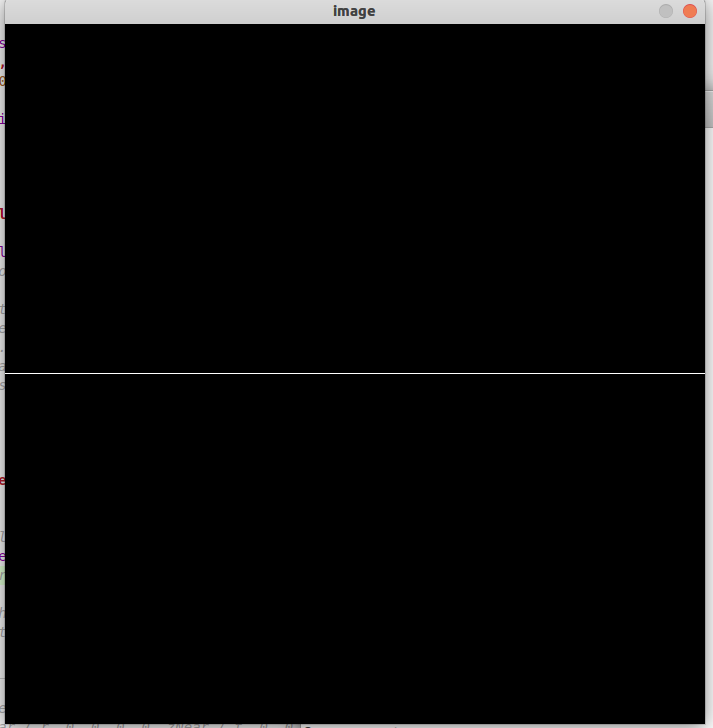
\includegraphics[width=1\textwidth]{job1.png}
    \caption{任务一图片}
\end{figure}
\indent{\fangsong 结果解释,只截取了三角形$x\in [-1,1],y\in [-1,1]$的部分,而原图像在该部分只有一条$y=0$直线,故在屏幕中央贯穿整个屏幕}

\section{\kaishu Job2、构建透视投影矩阵,将编译运行结果截图,并简述一下矩阵是如何构建。}
\indent{\fangsong 结果如下}
\begin{figure}[H]
    \centering
    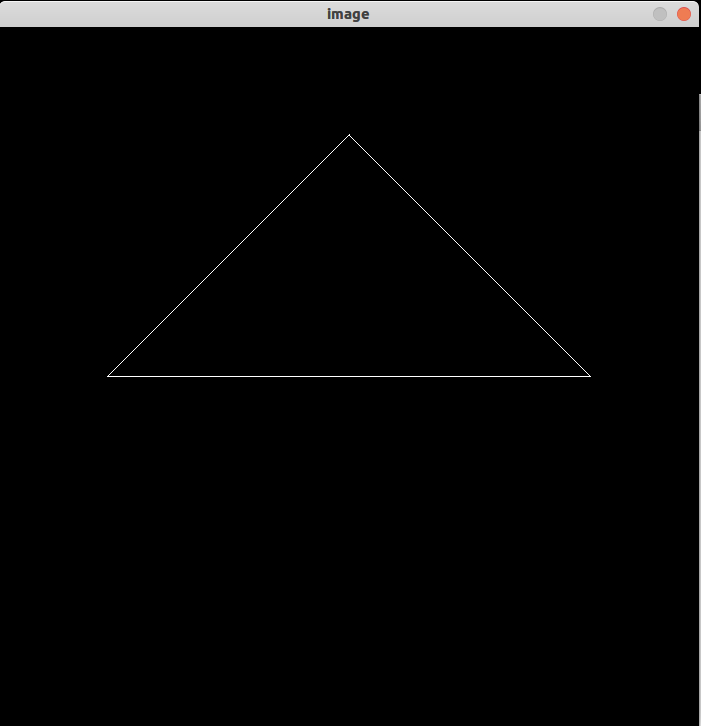
\includegraphics[width=1\textwidth]{job2.png}
    \caption{任务二图片}
\end{figure}
\indent{\fangsong 现在说明矩阵构建原理。最基本原理如下图所示,就时把视角范围内的点映射到在近$z$平面$x\in [-1,1],y\in [-1,1]$的范围内}\par
\begin{figure}[H]
    \centering
    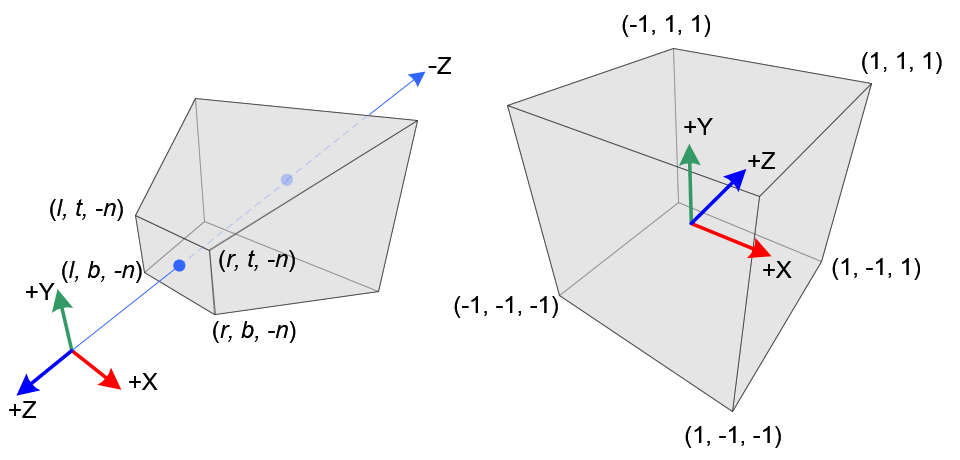
\includegraphics[width=1\textwidth]{gl_projectionmatrix01.png}
    \caption{原理图}
\end{figure}
\indent{\fangsong 在该图中具体来讲,就是把$x$轴的$[l, r]$ 映射到 $[-1, 1]$,把$y$轴的$[b, t]$ 也映射到 $[-1, 1]$,当然,都是$z=-n$处的平面}\par
\begin{figure}[H]
    \centering
    \subfigure[Top View of Frustum]{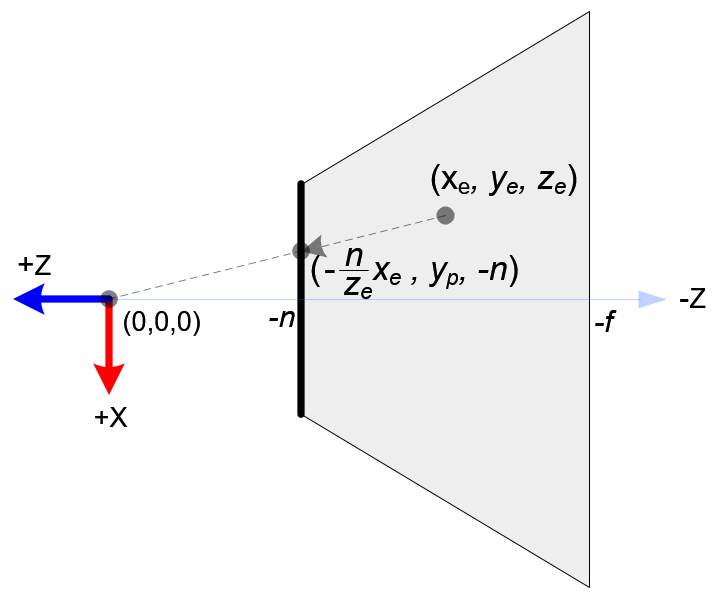
\includegraphics[width=0.4\textwidth]{gl_projectionmatrix03.png}}
    \subfigure[Side View of Frustum]{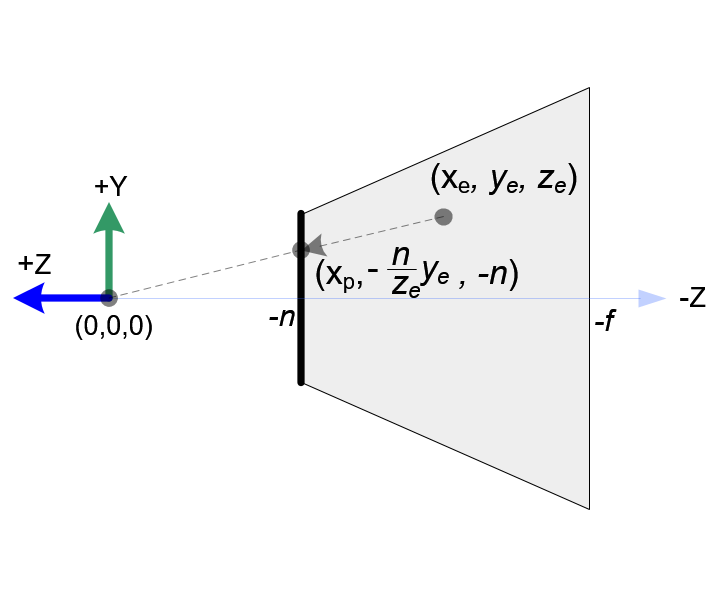
\includegraphics[width=0.4\textwidth]{gl_projectionmatrix04.png}}
    \caption{投影视图}
\end{figure}
\indent{\fangsong 根据相似三角形的原理,我们易知}
\begin{center}
    \begin{math}
        \left\{
        \begin{aligned}
            \frac{x_p}{x_e}=\frac{-n}{z_e}\quad \Rightarrow \quad x_p & =\frac{n \cdot x_e}{-z_e} \\
            \frac{y_p}{y_e}=\frac{-n}{z_e}\quad \Rightarrow \quad y_p & =\frac{n \cdot y_e}{-z_e} \\
        \end{aligned}
        \right.
    \end{math}
\end{center}
\indent{\fangsong 而$z_p$的值不容易求,所以我们直接求映射到$[-1,1]$的值,可以发现$z_e \in [-f,-n]$,对应$z_c \in [-1,1]$,故可知}
\begin{center}
    \begin{math}
        \left\{
        \begin{aligned}
            \frac{z_e-n}{f-n} & =-\frac{z_c+1}{2}              \\
            z_c               & =-\frac{z_e-n}{f-n} \cdot 2 +1
        \end{aligned}
        \right.
    \end{math}
\end{center}
\indent{\fangsong 而这里传入的$z_e$是正值,所以投影矩阵可写成}
\begin{center}
    \begin{math}
        \begin{aligned}
            \begin{vmatrix}
                \frac{n \cdot x_e}{-z_e\cdot r} \\
                \frac{n \cdot y_e}{-z_e\cdot t} \\
                -\frac{z_e-n}{f-n} \cdot 2 +1   \\
                1                               \\
            \end{vmatrix}
            =
            \begin{vmatrix}
                \cdot & \cdot & \cdot & \cdot \\
                \cdot & \cdot & \cdot & \cdot \\
                \cdot & \cdot & \cdot & \cdot \\
                \cdot & \cdot & \cdot & \cdot \\
            \end{vmatrix}
            \begin{vmatrix}
                x_e \\
                y_e \\
                z_e \\
                0   \\
            \end{vmatrix}
        \end{aligned}
    \end{math}
\end{center}
\par{\indent{\fangsong 但是这样发现不是线性组合,所以给左侧矩阵的$w_c$乘$-z_e$}}
\begin{center}
    \begin{math}
        \begin{aligned}
            \begin{vmatrix}
                \frac{n \cdot x_e}{ r}                     \\
                \frac{n \cdot y_e}{ t}                     \\
                (\frac{z_e-n}{f-n} \cdot 2 -1)\cdot (-z_e) \\
                -z_e                                       \\
            \end{vmatrix}
            =
            \begin{vmatrix}
                \cdot & \cdot & \cdot & \cdot \\
                \cdot & \cdot & \cdot & \cdot \\
                \cdot & \cdot & \cdot & \cdot \\
                \cdot & \cdot & \cdot & \cdot \\
            \end{vmatrix}
            \begin{vmatrix}
                x_e \\
                y_e \\
                z_e \\
                0   \\
            \end{vmatrix}
        \end{aligned}
    \end{math}
\end{center}
\par{\indent{\fangsong 但是这样发现仍然不是线性组合不是线性组合。这就很麻烦。只能换一种思路,$x$,$y$的坐标时定死的,但$z$的不是,只要变换完后能辨别出距离远近就可以,或者说,只要有一种从$z_e$到$z_c$的对应函数,并且是单调的,就可以满足这里可能存在的遮挡关系。所以可以想到以下的$z_c$算法,$-z_e \in [1/f,1/n]$,$z_c \in [-1,1]$}}
\begin{center}
    \begin{math}
        \begin{aligned}
            \frac{z_c+1}{2} & =-\frac{1/z_e-1/f}{1/n-1/f}      \\
            z_c             & =-\frac{-2nf-z_e(f+n)}{z_e(f-n)} \\
        \end{aligned}
    \end{math}
\end{center}
\indent{\fangsong 所以矩阵就变成了}
\begin{center}
    \begin{math}
        \begin{aligned}
            \begin{vmatrix}
                \frac{n \cdot x_e}{r}       \\
                \frac{n \cdot y_e}{t}       \\
                \frac{-2nf-z_e(f+n)}{(f-n)} \\
                -z_e                        \\
            \end{vmatrix}
            =
            \begin{vmatrix}
                \cdot & \cdot & \cdot & \cdot \\
                \cdot & \cdot & \cdot & \cdot \\
                \cdot & \cdot & \cdot & \cdot \\
                \cdot & \cdot & \cdot & \cdot \\
            \end{vmatrix}
            \begin{vmatrix}
                x_e \\
                y_e \\
                z_e \\
                0   \\
            \end{vmatrix}
        \end{aligned}
    \end{math}
\end{center}

\indent{\fangsong 容易解得矩阵为}
\begin{center}
    \begin{math}
        \begin{aligned}
            \begin{vmatrix}
                n/r & 0   & 0                & 0         \\
                0   & n/t & 0                & 0         \\
                0   & 0   & -\frac{f+n}{f-n} & -2fn(f-n) \\
                0   & 0   & -1               & 0         \\
            \end{vmatrix}
        \end{aligned}
    \end{math}
\end{center}
\section{\kaishu Job3、构建旋转变换矩阵,截图三张旋转结果,并简述一下矩阵是如何构建的}
\begin{figure}[H]
    \centering
    \subfigure[one]{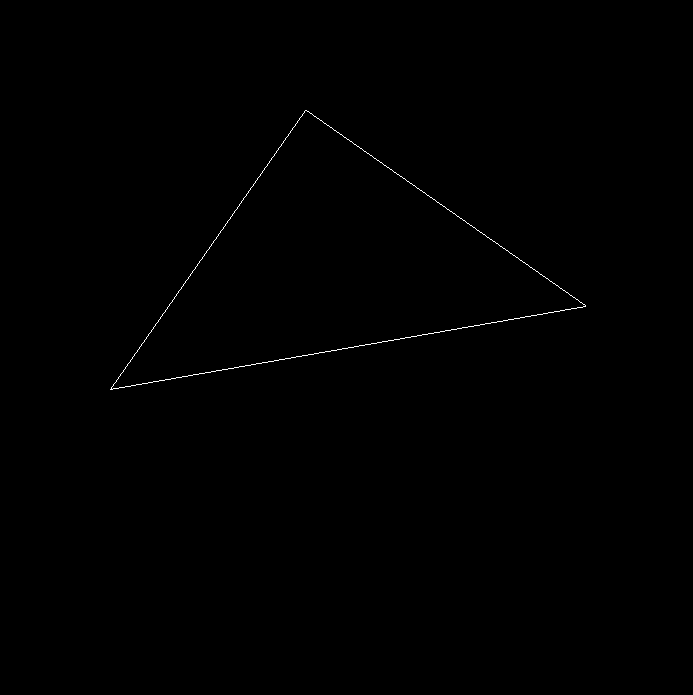
\includegraphics[width=0.3\textwidth]{job3_1.png}}
    \subfigure[two]{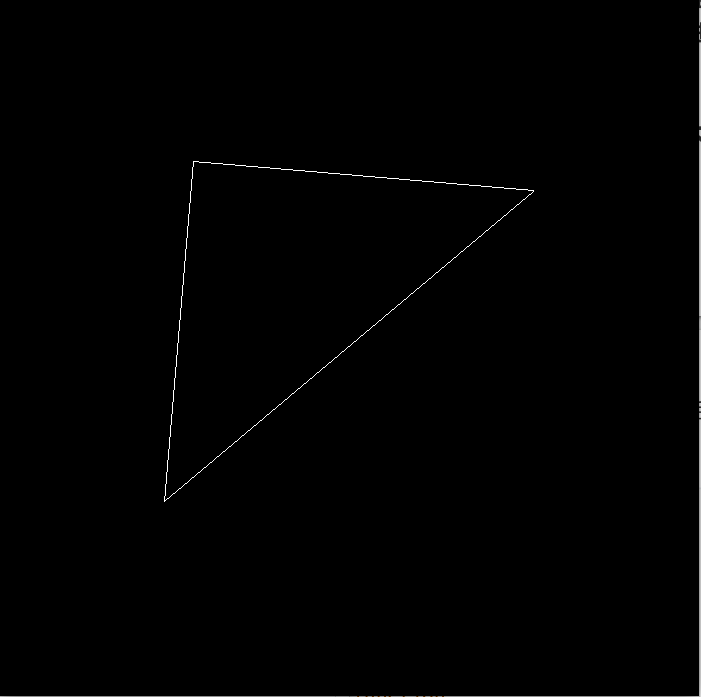
\includegraphics[width=0.3\textwidth]{job3_2.png}}
    \subfigure[three]{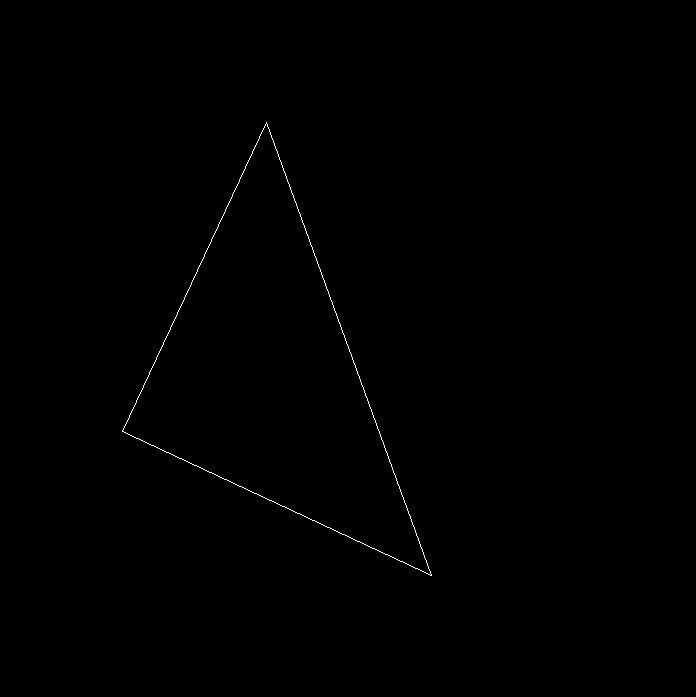
\includegraphics[width=0.3\textwidth]{job3_3.png}}
    \caption{投影视图}
\end{figure}
\indent{\fangsong 这个矩阵的构建就很简单了。首先$z$和$w$不变。只需要考虑$x$和$y$,假设变换后的坐标为$x'$,$y'$,设$r=\sqrt{x^2+y^2}$,$\alpha$为$(x,y)$与$(1,0)$所成的角,$\theta$为转动的角度,那么满足}
\begin{center}
    \begin{math}
        \begin{aligned}
            x  & =r\cos (\alpha)\quad y=r\sin(\alpha)             \\
            x' & =r\cos(\alpha+\theta)=\cos(\theta)x-\sin(theta)y \\
            y' & =r\sin(\alpha+\theta)=\sin(\theta)x+\cos(theta)y \\
        \end{aligned}
    \end{math}
\end{center}
\indent{\fangsong 容易解得矩阵为}
\begin{center}
    \begin{math}
        \begin{aligned}
            \begin{vmatrix}
                \cos(\theta) & -\sin(theta) & 0 & 0 \\
                \sin(\theta) & \cos(theta)  & 0 & 0 \\
                0            & 0            & 1 & 0 \\
                0            & 0            & 0 & 1 \\
            \end{vmatrix}
        \end{aligned}
    \end{math}
\end{center}
\section{\kaishu Job4、谈谈你对四维齐次坐标的理解}
\indent{\fangsong 一方面,如果只有三维,就不只用一个矩阵能构建出能对点进行平行变换的操作,虽然多加一维向量也可以做到,但是这样会非常不美观,而且有很多操作的时候,矩阵相乘进行化简也不容易实现。所以提出四维坐标,最后一维$w$就可以用来用作平移的常量。如果让我想,我就直接把最后一维设为$0$或$1$。$1$表示点,$0$表示向量。但是并不是这样,实际上,当$w\neq 0$ 时,四维坐标映射到对应的三维点为$x/w,z/w,z/w$。这个东西看起来没什么用,但时就如job2中构建投影矩阵中用到的法那个法一样,如果没有这样,那个变换就不能成为线性变换,从而导致无解。而关于为什么$1$表示点,$0$表示向量,可以想象作平移时候,点时可以移动的,而向量移动后完全不改变本身的属性}


% \section{\kaishu 标题}
% \subsection{次标题}
% \indent{\fangsong 文本}
% \begin{enumerate}
%     \item{\fangsong{列举}}
% \end{enumerate}
% \begin{lstlisting}[language=sql]
%     code
% \end{lstlisting}
% %换行公式对其
% \begin{center}
%     \begin{math}
%         \begin{aligned}
%             H(D|A) & =\sum_{a \in A}p(a)H(D|A=a) \\
%             g(D,A) & =H(D)-H(D|A)                \\
%                    & \text{$H(D|A)$为条件熵}     \\
%                    & \text{$g(D,A)$为信息增益}   \\
%         \end{aligned}
%     \end{math}
% \end{center}
% %大括号多行公式
% \begin{center}
%     \begin{math}
%         \left\{
%         \begin{aligned}
%             \dot{y_1} & = y_3 -r                    \\
%             \dot{y_2} & = y_1                       \\
%             \dot{y_3} & = -3a(y_3-r)-3a^2y_1-a^3y_2 \\
%         \end{aligned}
%         \right.
%     \end{math}
% \end{center}

% 拆入图片
% \begin{figure}[H]
%     \centering
%     \includegraphics[width=0.5\textwidth]{流程图/0.2.png}
%     \caption{最小信息增益<=0.2}
% \end{figure}




\end{document}